\section{Implement and Test}

\subsection{Description}

\noindent\fbox{
	\parbox{\textwidth}{
		\textbf{5.} Select the SysML/UML model for your preferred architecture suggestions in \textbf{3.} Choose a part of the functionality including both hardware and software components to create a model and a testbench in HLS using SystemC or C-code. Simulate and validate your design model. \\\\
		Argue for your choice of modeling language and abstraction level of modeling. Use the reports from the HLS tool to evaluate performance of the design. Assess whether the design is able to fulfill your requirements and constraints.\\\\
		\textbf{6.} Implement and test a part of your system using the ZYBO platform including at least one IP core written and verified with the HLS tool.
	}
}\citepawesome{Bjerge2017}{2}
\\\\

\subsection{Float as a Datatype}\label{imp:floatprototype}
Throughout this project, it has not been stated how essential it is that the data worked on is as close to real values as possible. Using long double as the used datatype both for calculation and evaluation for the particle swarm optimization algorithm is preferred. This is the floating point with most precision supported in SystemC. Working with Vivado  however, it is known that only fix point as a datatype is supported. To keep it simple the students have created a test program in the Vivado HLS tool that uses floats as a datatype both for calculations and in data transfers, to check if it is possible to use floating point, without conversion, when trying to hardware accelerate. The program that will be introduced in this section is floatPrototype.\\

The minimal design of floatPrototype is a IP core that take in two inputs, of type float, make a simple calculation with the data and returns it as a float. The outcome will conclude whether all the basic building blocks of the desired functionality in the PSOS can be achieved or not. On Figure \ref{fig:floatprototype} is a basic drawing of the desired flow of the floatPrototype IP core.

\begin{figure}[H]
	\centering
	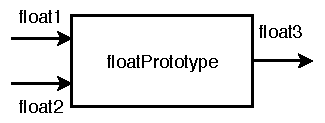
\includegraphics[width=0.5\linewidth]{diagram/floatPrototype}
	\caption{Figure showing the dataflow of floatPrototype.}
	\label{fig:floatprototype}
\end{figure}




\begin{lstlisting}[style=customc++, label={lst:floatPrototype.h}, caption={Simplified view of the header file of floatPrototype.}]
[...]
SC_MODULE(floatPrototypec){
[...]
  sc_in<float> float1;
  sc_in<float> float2;
  sc_out<float> float3;
  
  void multiply();
[...]
\end{lstlisting}

On Listing \ref{lst:floatPrototype.h} and \ref{lst:floatPrototype.cpp} is the SystemC implementation of floatPrototype, scaled down to the core of the IP core test. As can be seen on Listing \ref{lst:floatPrototype.h} the IP core that is being created has two float inputs, \texttt{float1} and \texttt{float2}, as well as a float output, \texttt{float3}. It has a function, \texttt{multiply()}, which simply multiplies \texttt{float1} with \texttt{float2} and writes the result onto \texttt{float3}.

\begin{lstlisting}[style=customc++, label={lst:floatPrototype.cpp}, caption={SystemC file of floatPrototype.}]
#include "floatPrototype.h"

void floatPrototypec::multiply(){
  #pragma HLS resource core=AXI4LiteS metadata="-bus_bundle slv0" variable=float1
[...]
  float3.write( float1.read() * float2.read() );
}
\end{lstlisting}

A simulation of the code is constructed and conducted in the Vivado HLS tools. The specific test is not included in this section. If study of the test is desired, the reader is referred to the HLS appendix that can be found in the "appendix.zip". The outcome of the test suit is the expected outcome in the case that the program functions using floats. The summary after the synthesis of floatPrototype can be seen on Figure \ref{fig:floatprototypesynthesissummary}.\\

\begin{figure}[H]
	\centering
	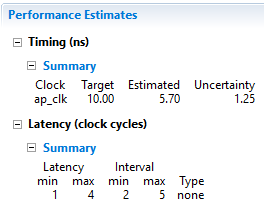
\includegraphics[width=0.428\linewidth]{diagram/floatPrototype_performance_summary}
	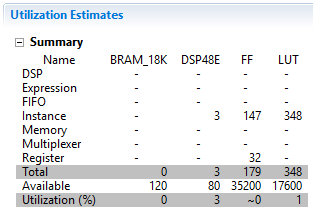
\includegraphics[width=0.5\linewidth]{diagram/floatPrototype_synthesis_summary}
	\caption{Autogenerated summary after synthesis of floatPrototype}
	\label{fig:floatprototypesynthesissummary}
\end{figure}


To further elaborate upon the float as a datatype test, the floatPrototype is exported as an RTL (Register-transfer level) from the Vivado HLS tool, and included into a simple program. The program has tests that are conducted to check whether it is possible to utilize floats in an IP core with the datatype being transferred directly. The open block design in Vivado can be seen on Figure \ref{fig:vivadoblockdesignwithipcore}.\\

\begin{figure}[H]
	\centering
	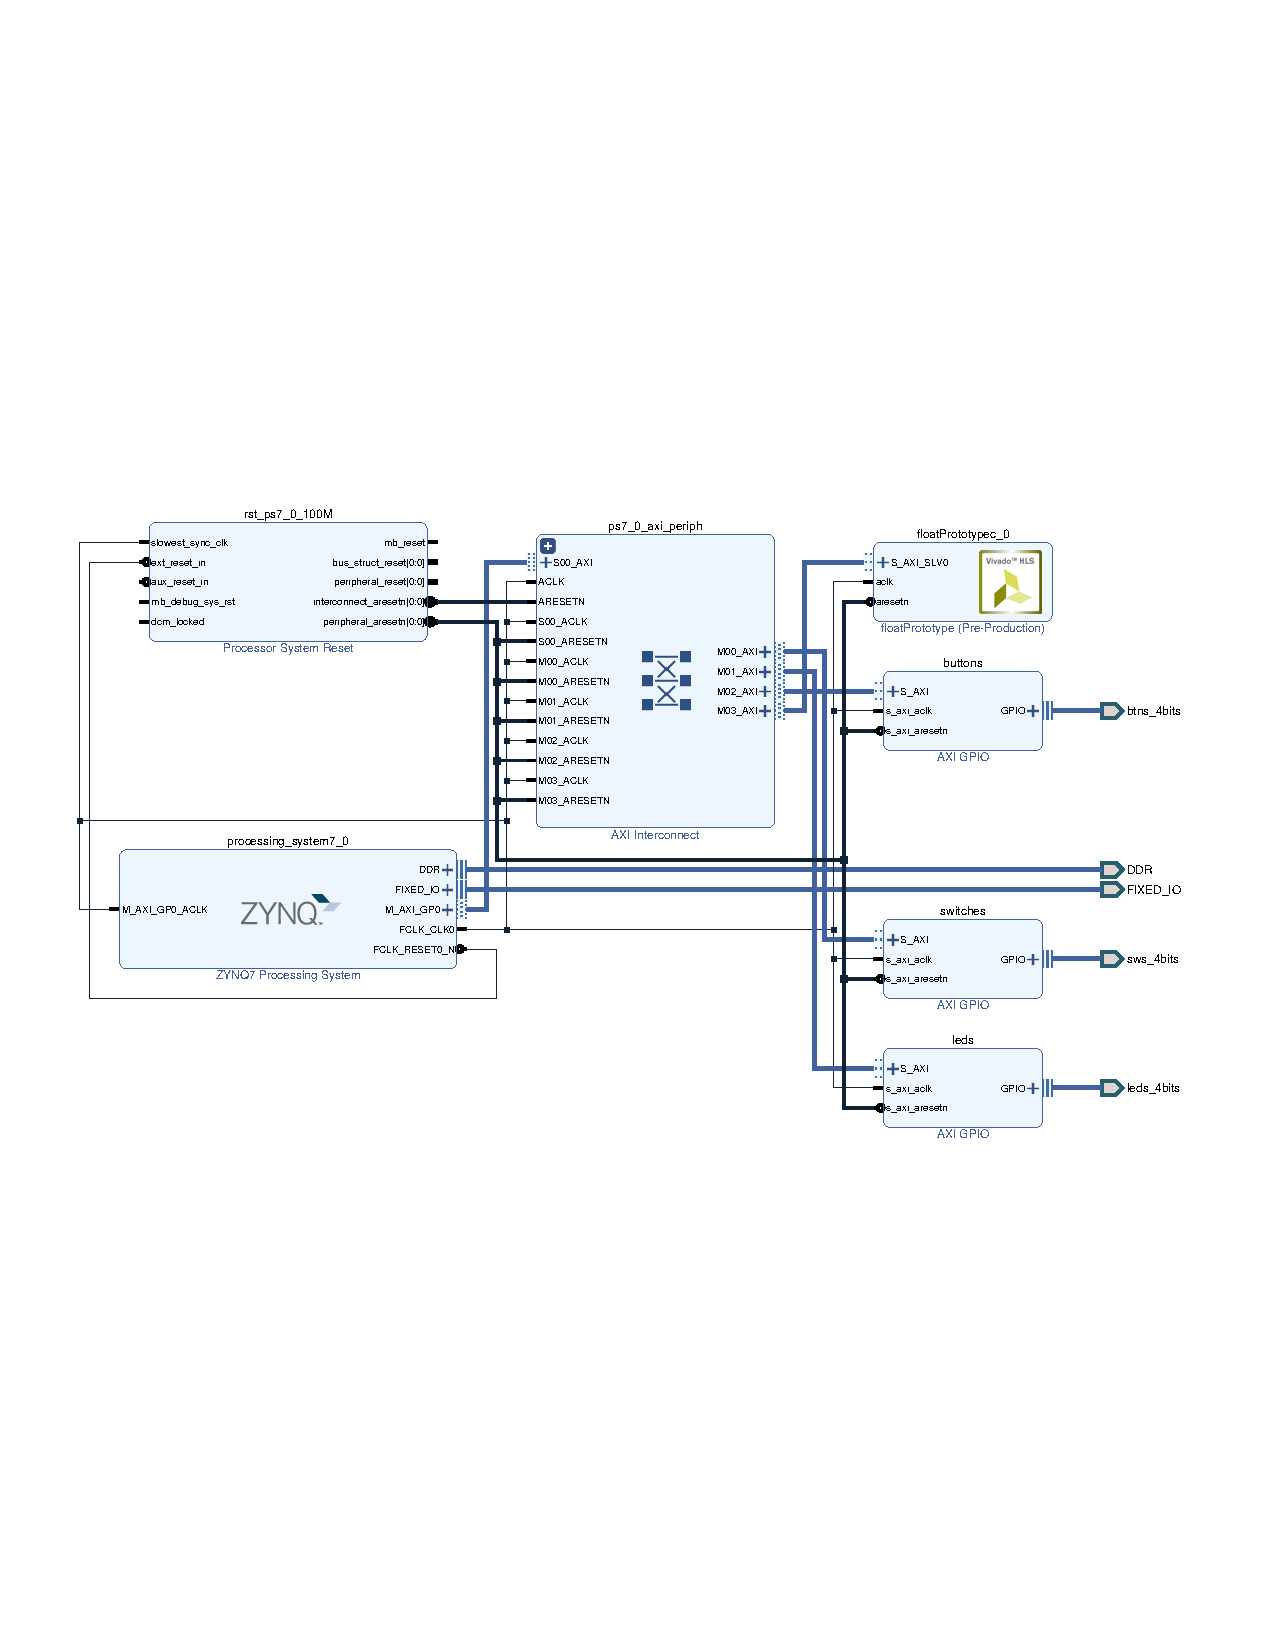
\includegraphics[trim={0 240 0 240},clip,width=1\linewidth]{diagram/VivadoBlockDesign_with_ip_core}
	\caption{Vivado open block design with floatPrototype as an IP core.}
	\label{fig:vivadoblockdesignwithipcore}
\end{figure}

At first glance it doesn't seem possible to send floats directly to and from the IP core, instead the core communicates using u32's in it's Axi Lite interface. Since a float use 32bits like an u32 it is possible to cheat the system to think that the datatype send is a u32, by making a u32 pointer point at a float object, when in fact it is a float. This is a bit of a hack, telling the system that it is of another datatype than what it is. By testing the IP core with a specific input values the output show that the IP core does indeed use floats. Results of a testprogram, performed on the Zybo board, can be seen on Figure \ref{fig:floatmultiply}.\\

\begin{figure}[H]
	\centering
	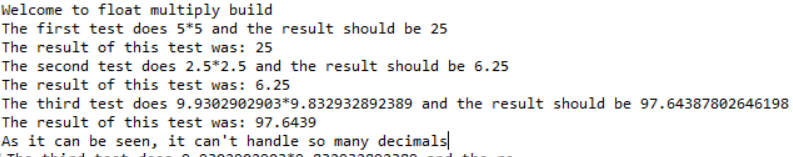
\includegraphics[trim={0 4 0 0},clip,width=0.8\linewidth]{diagram/floatMultiply}
	\caption{Result of floatPrototype IP core test, run on Zybo Board.}
	\label{fig:floatmultiply}
\end{figure}


With these tests conducted, it can be verified that it is indeed possible to hardware accelerate mathematical expressions in hardware.

\clearpage
\subsection{Vivado HLS}
With the knowledge acquired from section \ref{imp:floatprototype} \nameref{imp:floatprototype} the creation of a Particle Swarm Optimization algorithm on hardware seems possible, however dependent on the problem to solve it may be incredibly demanding. The problem that was chosen to use as a test is the "peaks" function\citepawesome{Chong2013}{290} and the algorithm that was implemented was first tested and verified in matlab and can be found in the appendix folder.\\

To see the complete code, the reader is referred to the appendix where the complete HLS code can be found.\\

In the design of the particles it is known that there will be two bottlenecks in which data can be problematic to handle. The first is the construction of a random value, it is not possible to create a random value inside an IP core with the HLS tools. Therefore the used Zynq CPU or another interface is needed to create a random value. This feature is abstracted away in this concept to simplify the project, but it is a known bottleneck that can slow the particles down. The second bottleneck is the global best solution after each iteration of movement of the particles. A central or master unit needs to check which solution of all the particles are the best solution, a simple version of this is implemented however this is a part of the system that can be heavily optimized in future versions of the system.\\

The PSOS HLS is divided into two different classes, a Particle and a ParticleMaster class. The Particles are doing the individual particle calculations while the master is the global calculation. The master also handles the communication to and from the Zynq CPU. On Figure \ref{fig:psoshlsconnections} the connections of the HLS component are shown.\\

\begin{figure}[H]
	\centering
	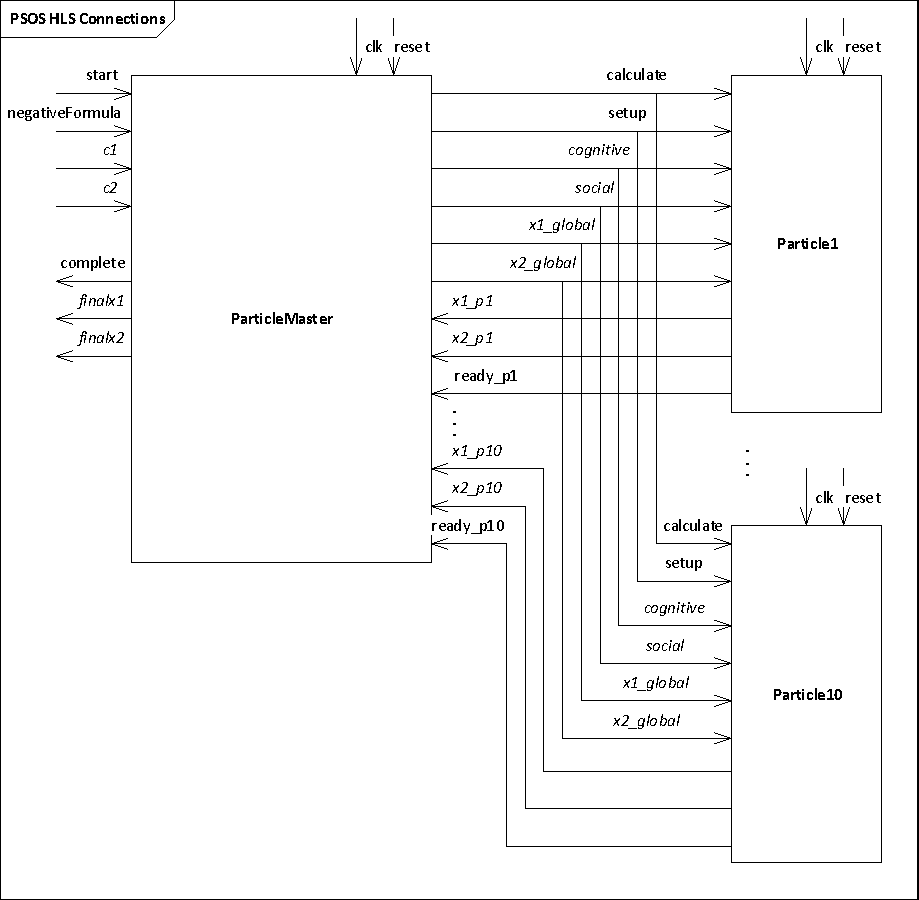
\includegraphics[width=0.7\linewidth]{diagram/psos_hls_connections}
	\caption{Diagram showing the connections of the HLS program. Normal text indicate that the datatype transfered is a boolean. Italic text indicate that the datatype transfered is a float.}
	\label{fig:psoshlsconnections}
\end{figure}

\subsubsection{ParticleMaster}

The ParticleMaster has two threads running. \texttt{Setup} and \texttt{ReadCalculations}. \texttt{Setup} awaits the \textit{start} connection to go high. When this event occurs it will start to setup the ten particles that is attached to it with the different variables that are used in the particle swarm optimization algorithm. When this has been done it starts the particles by letting the \textit{setup} connection go high. The code of the \texttt{Setup} can be seen in Listing \ref{lst:particlemaster_setup}.\\

\begin{lstlisting}[style=customc++, label={lst:particlemaster_setup}, caption={Setup thread of ParticleMaster.}]
void particlemaster::Setup(){
  while(true){
    while(!start.read() || setupDone){
      wait();
    }

    setup.write(false);
    setupDone = false;
    wait();

    // reading and setting up c1 and c2
    cognitive.write(c1.read());
    social.write(c2.read());
    wait();

    // Checking if we are looking for maximum or minimum and writing it
    negFormula = negativeFormula.read();
    wait();
    maximum.write(negFormula);
    wait();

    iterations = 60;
    setupDone = true;

    setup.write(true);
    wait();
  }
}
\end{lstlisting}

\texttt{ReadCalculations} awaits that all the particles are done with their calculation of each iteration before checking which of the particle has the best global position. If it has not run all the iterations through it will continue to make the particles calculate a new position after giving them the global best position. After the last iteration it will send the best position found back through the \textit{finalx1} and \textit{finalx2} connections and end with setting the \textit{complete} connection high as well. The code can be seen on Listing \ref{lst:particlemaster_readcalculations}.\\

\begin{lstlisting}[style=customc++, label={lst:particlemaster_readcalculations}, caption={ReadCalculations thread of ParticleMaster.}]
void particlemaster::ReadCalculations(){
  while(true){
    while(!(ready_p1.read() && ready_p2.read() && ready_p3.read() && ready_p4.read() && ready_p5.read() && ready_p6.read() && ready_p7.read() && ready_p8.read() && ready_p9.read() && ready_p10.read())){
      wait();
    }

    // Read values
    float x1s[10];
    float x2s[10];

    x1s[0] = x1_p1.read();
    x2s[0] = x2_p1.read();
    wait();
[...]
    x1s[9] = x1_p10.read();
    x2s[9] = x2_p10.read();
    wait();

    calculate.write(false);
    wait();

    float bestValue = Equation(x1_best, x2_best);

    for (int i = 0; i < sizeof(x1s); i++) {
      #pragma HLS INLINE
      if(Equation(x1s[i],x2s[i]) < bestValue)
      {
        bestValue = Equation(x1s[i],x2s[i]);
        x1_best = x1s[i];
        x2_best = x2s[i];
        wait();
      }
    }

    iterations--;

    if(iterations > 0)
    {
      x1_global.write(x1_best);
      x2_global.write(x2_best);
      wait();

      calculate.write(true);
      wait();
    }
    else
    {
      finalx1.write(x1_best);
      finalx2.write(x2_best);
      wait();

      complete.write(true);
      wait();
    }
  }
}
\end{lstlisting}

\subsubsection{Particle}
The ParticleMaster has ten particles attached. This is hardcoded as of now, but should be more than enough to create a proof of concept.\\

Like the ParticleMaster, each particle has two threads; \texttt{Setup} and \texttt{Execute}. Like the \texttt{Setup} thread from ParticleMaster, this thread uses the data communicated from the ParticleMaster to the Particles, to setup the different variables that can be modified. in this case it is only possible to change $c1$ and $c2$ which are the cognitive and social modifiers of the PSO. When the particles are setup they will set their start position at a random value with a random velocity. When this have been done it sends back the position coordinates to the master, through the \textit{x1\_out} and \textit{x2\_out} connections, and sets the \textit{ready} connection to high afterwards. Code can be seen on Listing \ref{lst:particle_setup}.\\

The particle is then setup and ready to start using execute.

\clearpage


\begin{lstlisting}[style=customc++, label={lst:particle_setup}, caption={Setup thread of Particle.}]
void particles::Setup(){
  while(true){
    while(!setup.read() || setupDone){
      wait();
    }

    ready.write(false);
    wait();

    setupDone = false;
    calculationDone = false;

    w = 0.8;
    ax = 10;
    av = 1;

    negativeFormula = maximum.read();
    c1 = cognitive.read();
    c2 = social.read();

    wait();

    // Make first position and velocity
    x1 = Random_position(0,ax);
    x2 = Random_position(0,ax);

    v1 = Random_velocity(av);
    v2 = Random_velocity(av);

    // Set first position as best position
    x1_best = x1;
    x2_best = x2;

    x1_out.write(x1);
    x2_out.write(x2);
    wait();

    setupDone = true;
    ready.write(true);
    wait();
  }
}
\end{lstlisting}

\texttt{Execute} awaits the internal \texttt{setupDone} flag as well as the \textit{calculate} connection to go high before starting the calculation process. The calculation process that is followed, is the standard equation of PSO shown in Equation \ref{eq:pso}.

\begin{equation}\label{eq:pso}
v_{i}(t+1)=wv_{i}(t)+c_{1}r_{1}(\hat{x}_{i}(t)-x_{i}(t))+c_{2}r_{2}(g(t)-x_{i}(t))
\end{equation}\\

Every time a new position has been calculated it is tested whether or not the position is a more optimized position than the old best cognitive position. If so, the particle overrides the old best position with the new position. After this process, the Particle set the \textit{ready} communication to high and awaits the next command.

\clearpage

\begin{lstlisting}[style=customc++, label={lst:particle_execute}, caption={Execute thread of Particle.}]
void particles::Execute(){
  while(true){
    while(!(setupDone && calculate.read()) || calculationDone){
      if(!calculate.read())
      {
        calculationDone = false;
      }
      wait();
    }

    ready.write(false);
    wait();

    v1 = w*v1 + c1*Randval()*(x1_best-x1) + c2*Randval()*(x1_global.read()-x1);
    v2 = w*v2 + c1*Randval()*(x2_best-x2) + c2*Randval()*(x2_global.read()-x2);
    wait();

    x1 = x1+v1;
    x2 = x2+v2;

    if (Equation(x1,x2) < Equation(x1_best,x2_best))
    {
      x1_best = x1;
      x2_best = x2;
    }

    x1_out.write(x1);
    x2_out.write(x2);

    calculationDone = true;

    ready.write(true);
    wait();
  }
}
\end{lstlisting}

After synthesizing the SystemC model, it is obvious that the IP Core is far too demanding for the FPGA on the Zybo board in this project. Summaries of the results can be seen on Figure \ref{fig:psossynthesissummary}. These results will be elaborated further upon in section \ref{sc:conclusion} \nameref{sc:conclusion}, on page \pageref{sc:conclusion}.

\begin{figure}[H]
	\centering
	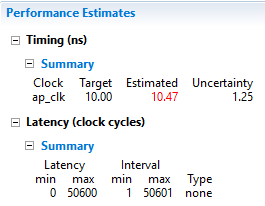
\includegraphics[width=0.415\linewidth]{diagram/psos_performance_summary}
	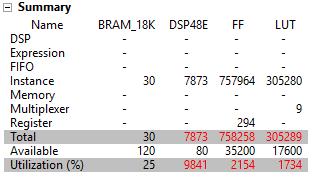
\includegraphics[width=0.5\linewidth]{diagram/psos_synthesis_summary}
	\caption{Autogenerated summary after synthesis of PSOS HLS.}
	\label{fig:psossynthesissummary}
\end{figure}

\clearpage

\subsection{Vivado}
The implementation of the PSO through the HLS tool have shown that the Zybo board used in this project doesn't have the necessary FPGA to implement the IP core on the board. Therefore the implementation of the GUI design won't include the IP Core generated in the Open Block design. The PSO have been abstracted away to test the design on the board.\\

This section show the implementation of the different software patterns mentioned in section \ref{designpatterns} \nameref{designpatterns}, page \pageref{designpatterns}, on the Zynq CPU. The design makes use of the GPIO ports to access the hardware buttons and switches, to control the state of the PSOS, as shown on Figure \ref{fig:smdguistate}, on page \pageref{fig:smdguistate}. The buttons are used to control the actions in the application ActionUp, ActionDown, ActionNext and ActionStart. The switches are used to control the different of the PSOS; Setup, FindMinima and FindMaxima. The open block design used to test the GUI software can be seen on Figure \ref{fig:vivadoblockdesign}.

\begin{figure}[H]
	\centering
	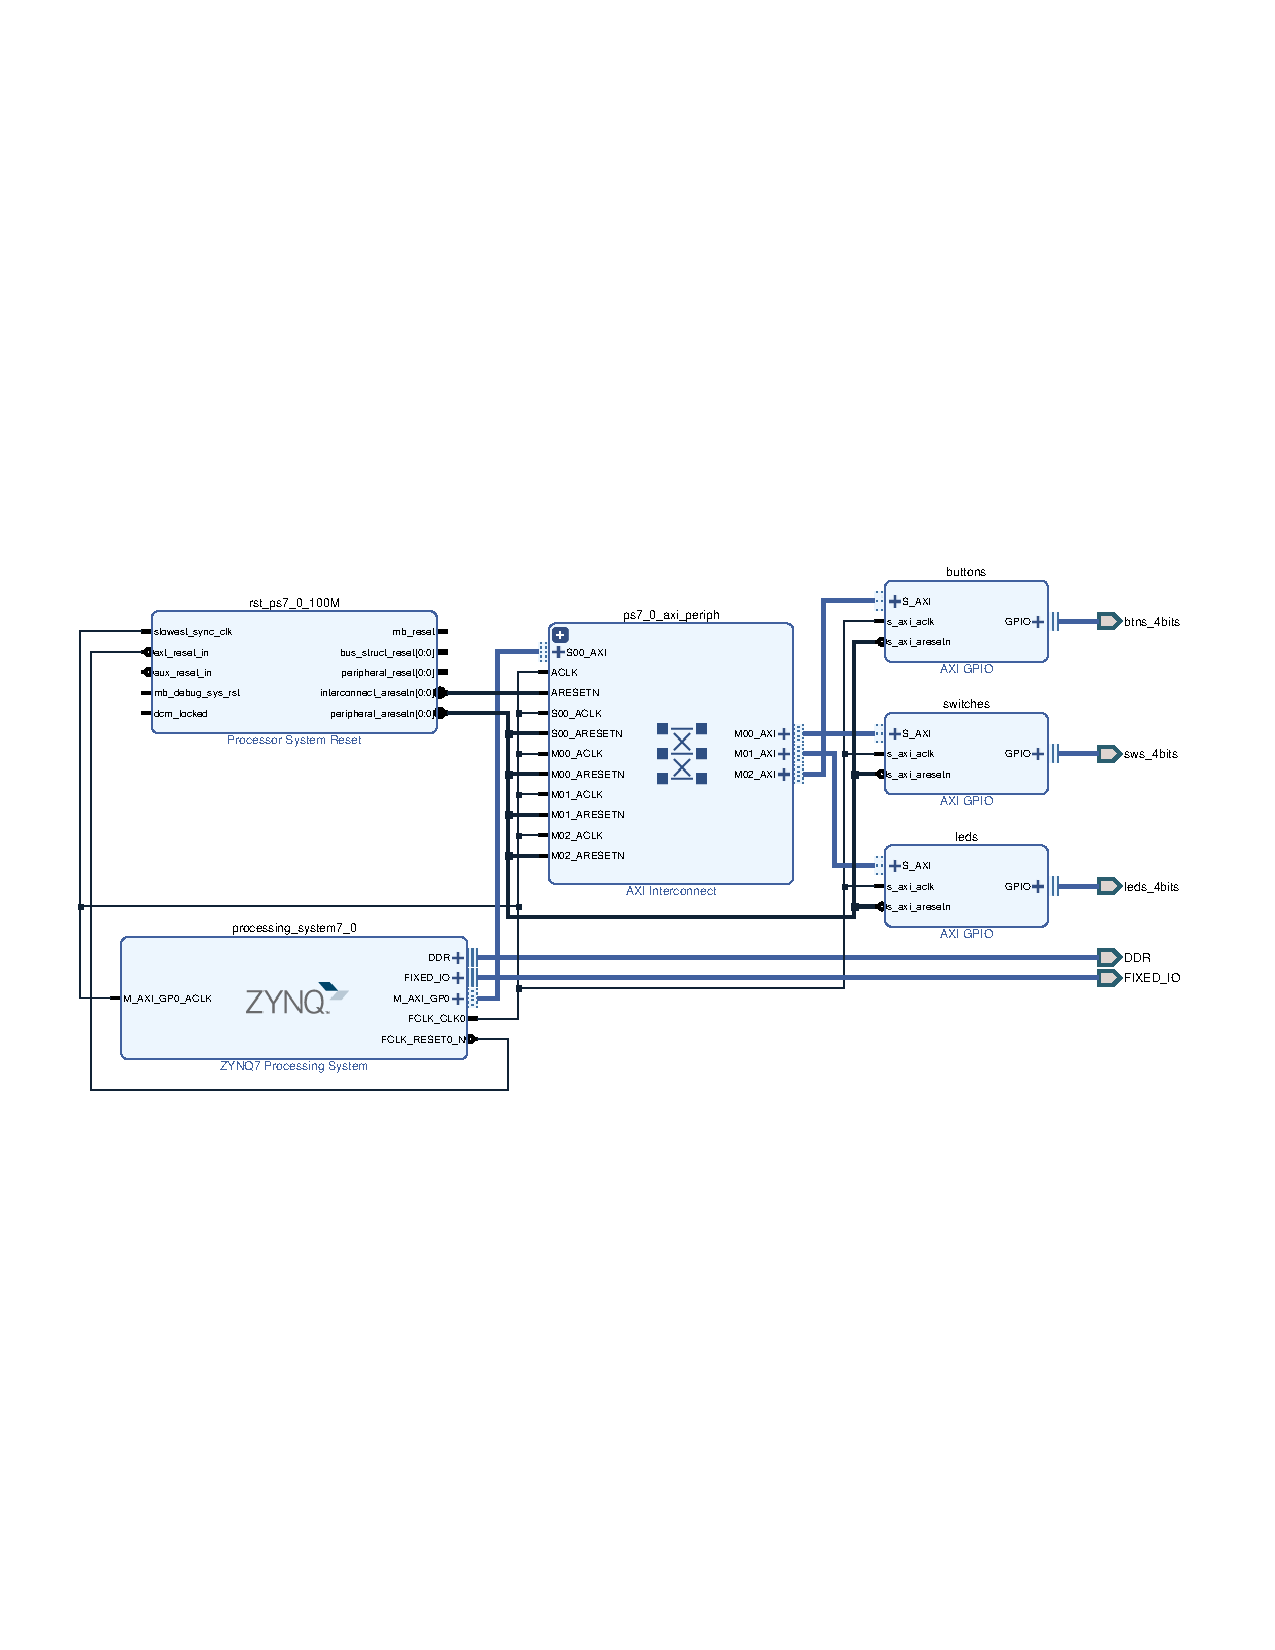
\includegraphics[trim={0 260 0 260},clip,width=1\linewidth]{diagram/VivadoBlockDesign}
	\caption{Vivado open block design of design used to test GUI software.}
	\label{fig:vivadoblockdesign}
\end{figure}

The Software is made using FreeRTOS, where the mainThread controls the application. As it can be seen in Listing \ref{lst:mainthread_run} it initializes the buttons and switches, and starts checking on button and switch events. In the case a new event occurs, it sends a command via command pattern to the current state.

\begin{lstlisting}[style=customc++, label={lst:mainthread_run}, caption={MainThread run thread.}]
[...]
void MainThread::run(){
  xil_printf("Welcome to Particle Swarm Optimization Embedded \r\n");

  XGpio dip, push;

  XGpio_Initialize(&dip, XPAR_SWITCHES_DEVICE_ID);
  XGpio_SetDataDirection(&dip, 1, 0xffffffff);

  XGpio_Initialize(&push, XPAR_BUTTONS_DEVICE_ID);
  XGpio_SetDataDirection(&push, 1, 0xffffffff);

  xil_printf("Use the switches to control the menu \r\n");

  _context = new Context;
  //Transitions
  FindMinimaCommand findMinimaCommand = FindMinimaCommand(_context);
  FindMaximaCommand findMaximaCommand = FindMaximaCommand(_context);
  ReturnResultCommand returnResultCommand = ReturnResultCommand(_context);

  while (true){
    switch (XGpio_DiscreteRead(&dip, 1)) {
      case 0:
        returnResultCommand.returnedResult = 10;
        returnResultCommand.Execute();
        buttonCommand(_context, XGpio_DiscreteRead(&push, 1));
        break;
      case 1:
        findMinimaCommand.Execute();
        buttonCommand(_context, XGpio_DiscreteRead(&push, 1));
        break;
      case 2:
        findMaximaCommand.Execute();
        buttonCommand(_context, XGpio_DiscreteRead(&push, 1));
        break;
      default:
        break;
    }
    for (int i = 0; i < 9999; ++i);
  }
}
[...]
\end{lstlisting}

As mentioned in section \ref{dp:command} \nameref{dp:command}, on page \pageref{dp:command}, the usage of the GOF Command Pattern will be used to execute commands on the state pattern. An example of an implemented command can be seen on Listing \ref{lst:findmaxima_command}.

\begin{lstlisting}[style=customc++, label={lst:findmaxima_command}, caption={FindMaxima command implementation.}]
[...]
FindMaximaCommand::FindMaximaCommand(Context* c) {
  _context = c;
}
void FindMaximaCommand::Execute(){
  _context->GoMaxima();
}
\end{lstlisting}

In section \ref{dp:state} \nameref{dp:state}, on page \pageref{dp:state}, it is decided that the usage of GOF State Pattern shall be utilized to maintain the states of the GUI. On Listing \ref{lst:setup_state} the implementation of an action and a transition can be seen as an example from the Setup state. \texttt{ActionUp()} changes the internal value $c1$, \texttt{GoMaxima(context*)} changes the state from \textit{Setup} to \textit{FindMaxima}.

\begin{lstlisting}[style=customc++, label={lst:setup_state}, caption={Actions implemented in the Setup state.}]
[...]
void Setup::ActionUp(){
  if(toggle == true)
  {
    std::cout << "ActionUp called c1: " << ++c1 << std::endl;
  } else {
    std::cout << "ActionUp called c2: " << ++c2 << std::endl;
  }
}
void Setup::GoMaxima(Context* c){
  std::cout << "GoMaxima" << std::endl;
  ChangeState(c, new FindMaxima());
}
[...]
\end{lstlisting}

Because of the need to remember the values $c1$ and $c2$ inside the Setup state, the Setup state is implemented as a singleton. This implements deep history into the class as stated in section \ref{dp:singleton} \nameref{dp:singleton}, on page \pageref{dp:singleton}. The implementation of the singleton pattern can be seen on Listing \ref{lst:setup_singleton}.

\begin{lstlisting}[style=customc++, label={lst:setup_singleton}, caption={Singleton implementation in the Setup state.}]
[...]
Setup* Setup::_instance = 0;

Setup* Setup::Instance() {
  if (_instance == 0) {
    _instance = new Setup();
  }

  std::cout << "Please set c1 and c2" << std::endl;
  return _instance;
}

Setup::Setup() {
  toggle = true;
  c1 = 1;
  c2 = 1;
}
[...]
\end{lstlisting}

Testing the functionality of the software on the Zybo Board gives the expected result and the output from the console can be seen in Figure \ref{fig:particleswarmoptimizationembedded}.

\begin{figure}[H]
	\centering
	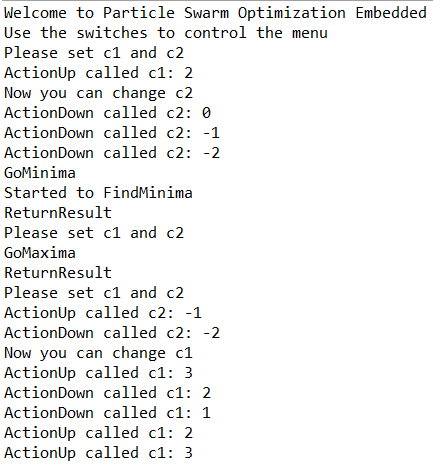
\includegraphics[trim={0 0 0 4},clip,width=0.45\linewidth]{diagram/ParticleSwarmOptimizationEmbedded}
	\caption{Console output of Vivado test program.}
	\label{fig:particleswarmoptimizationembedded}
\end{figure}
